\documentclass[a4paper,11pt,fleqn]{article}

\usepackage[left=1cm,right=0.5cm,top=0.5cm,bottom=2cm]{geometry}

\usepackage{bfcours}
\usepackage{bfcours-fonts}
%\usepackage{bfcours-fonts-dys}

\def\rdifficulty{1}
\setrdexo{%left skip=1cm,
display exotitle,
exo header = tcolorbox,
%display tags,
skin = bouyachakka,
lower ={box=crep},
display score,
display level,
save lower,
score=\points,
level=\rdifficulty,
overlay={\node[inner sep=0pt,
anchor=west,rotate=90, yshift=0.3cm]%,xshift=-3em], yshift=0.45cm
at (frame.south west) {\thetags[0]} ;}
]%obligatoire
}
\setrdcrep{seyes, correction=true, correction color=monrose, correction font = \large\bfseries}

\newcommand{\tikzinclude}[1]{%
    \stepcounter{tikzfigcounter}%
    \csname tikzfig#1\endcsname
}

\newcommand{\tikzfiggGnt}{
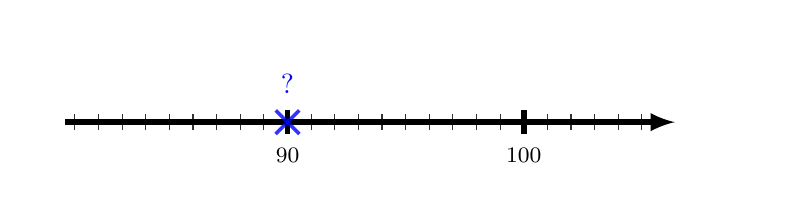
\begin{tikzpicture}[baseline,scale = 0.6]
	
		\tikzset{
		  point/.style={
			thick,
			draw,
			cross out,
			inner sep=0pt,
			minimum width=5pt,
			minimum height=5pt,
		  },
		}
		\clip (-1,-1) rectangle (15,2);
			\draw[color ={black},line width = 2,>=latex,->] (-0.2,0)--(12.7,0);
		\draw[color ={black},opacity = 0.8] (0,-0.17)--(0,0.17);
		\draw[color ={black},opacity = 0.8] (0.5,-0.17)--(0.5,0.17);
		\draw[color ={black},opacity = 0.8] (1,-0.17)--(1,0.17);
		\draw[color ={black},opacity = 0.8] (1.5,-0.17)--(1.5,0.17);
		\draw[color ={black},opacity = 0.8] (2,-0.17)--(2,0.17);
		\draw[color ={black},opacity = 0.8] (2.5,-0.17)--(2.5,0.17);
		\draw[color ={black},opacity = 0.8] (3,-0.17)--(3,0.17);
		\draw[color ={black},opacity = 0.8] (3.5,-0.17)--(3.5,0.17);
		\draw[color ={black},opacity = 0.8] (4,-0.17)--(4,0.17);
		\draw[color ={black},line width = 2] (4.5,-0.25)--(4.5,0.25);
		\draw[color ={black},opacity = 0.8] (5,-0.17)--(5,0.17);
		\draw[color ={black},opacity = 0.8] (5.5,-0.17)--(5.5,0.17);
		\draw[color ={black},opacity = 0.8] (6,-0.17)--(6,0.17);
		\draw[color ={black},opacity = 0.8] (6.5,-0.17)--(6.5,0.17);
		\draw[color ={black},opacity = 0.8] (7,-0.17)--(7,0.17);
		\draw[color ={black},opacity = 0.8] (7.5,-0.17)--(7.5,0.17);
		\draw[color ={black},opacity = 0.8] (8,-0.17)--(8,0.17);
		\draw[color ={black},opacity = 0.8] (8.5,-0.17)--(8.5,0.17);
		\draw[color ={black},opacity = 0.8] (9,-0.17)--(9,0.17);
		\draw[color ={black},line width = 2] (9.5,-0.25)--(9.5,0.25);
		\draw[color ={black},opacity = 0.8] (10,-0.17)--(10,0.17);
		\draw[color ={black},opacity = 0.8] (10.5,-0.17)--(10.5,0.17);
		\draw[color ={black},opacity = 0.8] (11,-0.17)--(11,0.17);
		\draw[color ={black},opacity = 0.8] (11.5,-0.17)--(11.5,0.17);
		\draw[color ={black},opacity = 0.8] (12,-0.17)--(12,0.17);
		\draw (4.5,-0.7) node[anchor = center] {\footnotesize \color{black}{$90$}};
		\draw (9.5,-0.7) node[anchor = center] {\footnotesize \color{black}{$100$}};
		\draw[color ={blue},line width = 1.25,opacity = 0.8] (4.25,0.25)--(4.75,-0.25);\draw[color ={blue},line width = 1.25,opacity = 0.8] (4.25,-0.25)--(4.75,0.25);
		\draw (4.5,0.8) node[anchor = center, rotate=0] {\normalsize \color{blue}{$?$}};
	
	\end{tikzpicture}
}

\newcommand{\tikzfigUfpC}{
\begin{tikzpicture}[baseline,scale = 0.8]
	
		\tikzset{
		  point/.style={
			thick,
			draw,
			cross out,
			inner sep=0pt,
			minimum width=5pt,
			minimum height=5pt,
		  },
		}
		\clip (-1.5,-1) rectangle (5,4);
			\draw [color={black}] (2,-0.5) node[anchor = center,scale=1, rotate = 0] {8,5 cm};
		\draw [color={black}] (2,3.5) node[anchor = center,scale=1, rotate = 0] {8,5 cm};
		\draw [color={black}] (4.5,1.5) node[anchor = center,scale=1, rotate = 0] {?};
		\draw[color ={black}] (0,0)--(4,0);
		\draw[color ={black}] (4,0)--(4,3);
		\draw[color ={black}] (4,3)--(0,3);
		\draw[color ={black}] (0,3)--(0,0);
		\draw[color={black},line width = 0.5] (4,0)--(3.6,0)--(3.6,0.4)--(4,0.4)--cycle;
		\draw[color={black},line width = 0.5] (4,3)--(4,2.6)--(3.6,2.6)--(3.6,3)--cycle;
		\draw[color={black},line width = 0.5] (0,3)--(0.4,3)--(0.4,2.6)--(0,2.6)--cycle;
		\draw[color={black},line width = 0.5] (0,0)--(0,0.4)--(0.4,0.4)--(0.4,0)--cycle;
	
	\end{tikzpicture}
}

\newcommand{\tikzfigaETb}{
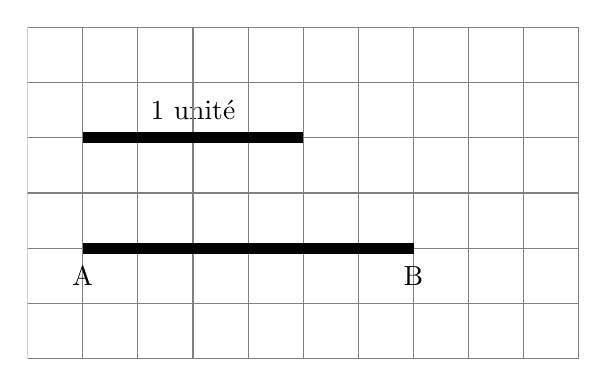
\begin{tikzpicture}[baseline,scale = 0.7]
	
		\tikzset{
		  point/.style={
			thick,
			draw,
			cross out,
			inner sep=0pt,
			minimum width=5pt,
			minimum height=5pt,
		  },
		}
		\clip (-1,-2) rectangle (9,4);
			\draw [color={black}] (2,2.5) node[anchor = center,scale=1, rotate = 0] {1 unité};
		\draw[color ={gray}] (-2,-2)--(-2,4);
		\draw[color ={gray}] (-1,-2)--(-1,4);
		\draw[color ={gray}] (0,-2)--(0,4);
		\draw[color ={gray}] (1,-2)--(1,4);
		\draw[color ={gray}] (2,-2)--(2,4);
		\draw[color ={gray}] (3,-2)--(3,4);
		\draw[color ={gray}] (4,-2)--(4,4);
		\draw[color ={gray}] (5,-2)--(5,4);
		\draw[color ={gray}] (6,-2)--(6,4);
		\draw[color ={gray}] (7,-2)--(7,4);
		\draw[color ={gray}] (8,-2)--(8,4);
		\draw[color ={gray}] (9,-2)--(9,4);
		\draw[color ={gray}] (-2,-2)--(9,-2);
		\draw[color ={gray}] (-2,-1)--(9,-1);
		\draw[color ={gray}] (-2,0)--(9,0);
		\draw[color ={gray}] (-2,1)--(9,1);
		\draw[color ={gray}] (-2,2)--(9,2);
		\draw[color ={gray}] (-2,3)--(9,3);
		\draw[color ={gray}] (-2,4)--(9,4);
		\draw[color ={black},line width = 4] (0,2)--(4,2);
		\draw[color ={black},line width = 4] (0,0)--(6,0);
		\draw [color={black}] (0,-0.5) node[anchor = center,scale=1, rotate = 0] {A};
		\draw [color={black}] (6,-0.5) node[anchor = center,scale=1, rotate = 0] {B};
	
	\end{tikzpicture}
}

\newcommand{\tikzfigeYEf}{
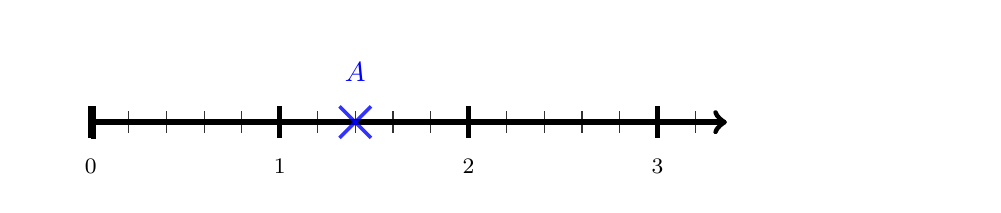
\begin{tikzpicture}[baseline,scale = 0.8]
	
		\tikzset{
		  point/.style={
			thick,
			draw,
			cross out,
			inner sep=0pt,
			minimum width=5pt,
			minimum height=5pt,
		  },
		}
		\clip (-1,-1) rectangle (14,1.5);
			\draw[color ={black},line width = 2,|->] (0,0)--(10.1,0);
		\draw[color ={black},line width = 2] (0,-0.25)--(0,0.25);
		\draw[color ={black},opacity = 0.8] (0.6,-0.17)--(0.6,0.17);
		\draw[color ={black},opacity = 0.8] (1.2,-0.17)--(1.2,0.17);
		\draw[color ={black},opacity = 0.8] (1.8,-0.17)--(1.8,0.17);
		\draw[color ={black},opacity = 0.8] (2.4,-0.17)--(2.4,0.17);
		\draw[color ={black},line width = 2] (3,-0.25)--(3,0.25);
		\draw[color ={black},opacity = 0.8] (3.6,-0.17)--(3.6,0.17);
		\draw[color ={black},opacity = 0.8] (4.2,-0.17)--(4.2,0.17);
		\draw[color ={black},opacity = 0.8] (4.8,-0.17)--(4.8,0.17);
		\draw[color ={black},opacity = 0.8] (5.4,-0.17)--(5.4,0.17);
		\draw[color ={black},line width = 2] (6,-0.25)--(6,0.25);
		\draw[color ={black},opacity = 0.8] (6.6,-0.17)--(6.6,0.17);
		\draw[color ={black},opacity = 0.8] (7.2,-0.17)--(7.2,0.17);
		\draw[color ={black},opacity = 0.8] (7.8,-0.17)--(7.8,0.17);
		\draw[color ={black},opacity = 0.8] (8.4,-0.17)--(8.4,0.17);
		\draw[color ={black},line width = 2] (9,-0.25)--(9,0.25);
		\draw[color ={black},opacity = 0.8] (9.6,-0.17)--(9.6,0.17);
		\draw (0,-0.7) node[anchor = center] {\footnotesize \color{black}{$0$}};
		\draw (3,-0.7) node[anchor = center] {\footnotesize \color{black}{$1$}};
		\draw (6,-0.7) node[anchor = center] {\footnotesize \color{black}{$2$}};
		\draw (9,-0.7) node[anchor = center] {\footnotesize \color{black}{$3$}};
		\draw[color ={blue},line width = 1.25,opacity = 0.8] (3.95,0.25)--(4.45,-0.25);\draw[color ={blue},line width = 1.25,opacity = 0.8] (3.95,-0.25)--(4.45,0.25);
		\draw (4.199999999999999,0.8) node[anchor = center, rotate=0] {\normalsize \color{blue}{$A$}};
	
	\end{tikzpicture}
}

\newcommand{\tikzfigocLB}{

\begin{tikzpicture}[baseline,scale = 0.3]

    \tikzset{
      point/.style={
        thick,
        draw,
        cross out,
        inner sep=0pt,
        minimum width=5pt,
        minimum height=5pt,
      },
    }
    \clip (-0.7,-2.7) rectangle (7.7,0.7);
    	
	 \filldraw[color={black},fill={black}] (0,0) circle (0.2);
	
	 \filldraw[color={black},fill={black}] (1,0) circle (0.2);
	
	 \filldraw[color={black},fill={black}] (2,0) circle (0.2);
	
	 \filldraw[color={black},fill={black}] (3,0) circle (0.2);
	
	 \filldraw[color={black},fill={black}] (4,0) circle (0.2);
	
	 \filldraw[color={black},fill={black}] (5,0) circle (0.2);
	
	 \filldraw[color={black},fill={black}] (6,0) circle (0.2);
	
	 \filldraw[color={black},fill={black}] (7,0) circle (0.2);
	
	 \filldraw[color={black},fill={black}] (0,-1) circle (0.2);
	
	 \filldraw[color={black},fill={black}] (1,-1) circle (0.2);
	
	 \filldraw[color={black},fill={black}] (2,-1) circle (0.2);
	
	 \filldraw[color={black},fill={black}] (3,-1) circle (0.2);
	
	 \filldraw[color={black},fill={black}] (4,-1) circle (0.2);
	
	 \filldraw[color={black},fill={black}] (5,-1) circle (0.2);
	
	 \filldraw[color={black},fill={black}] (6,-1) circle (0.2);
	
	 \filldraw[color={black},fill={black}] (7,-1) circle (0.2);
	
	 \filldraw[color={black},fill={black}] (0,-2) circle (0.2);
	
	 \filldraw[color={black},fill={black}] (1,-2) circle (0.2);
	
	 \filldraw[color={black},fill={black}] (2,-2) circle (0.2);
	
	 \filldraw[color={black},fill={black}] (3,-2) circle (0.2);
	
	 \filldraw[color={black},fill={black}] (4,-2) circle (0.2);
	
	 \filldraw[color={black},fill={black}] (5,-2) circle (0.2);
	
	 \filldraw[color={black},fill={black}] (6,-2) circle (0.2);
	
	 \filldraw[color={black},fill={black}] (7,-2) circle (0.2);

\end{tikzpicture}
}

\newcommand{\tikzfigfUFI}{
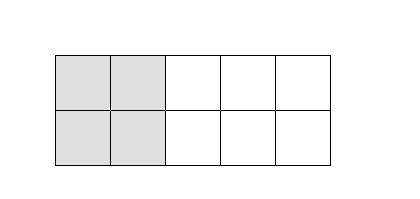
\begin{tikzpicture}[baseline,scale = 0.7]

    \tikzset{
      point/.style={
        thick,
        draw,
        cross out,
        inner sep=0pt,
        minimum width=5pt,
        minimum height=5pt,
      },
    }
    \clip (-0.5,-0.1) rectangle (6.1,2.5);
    	\draw[color={black},preaction={fill,color = {lightgray}, opacity = 0.5}] (0,0)--(2,0)--(2,2)--(0,2)--(0,2)--(0,2)--cycle;
	\draw[color ={black}] (0,0)--(0,2);
	\draw[color ={black}] (1,0)--(1,2);
	\draw[color ={black}] (2,0)--(2,2);
	\draw[color ={black}] (3,0)--(3,2);
	\draw[color ={black}] (4,0)--(4,2);
	\draw[color ={black}] (5,0)--(5,2);
	\draw[color ={black}] (0,0)--(5,0);
	\draw[color ={black}] (0,1)--(5,1);
	\draw[color ={black}] (0,2)--(5,2);

\end{tikzpicture}
}

\newcommand{\tikzfiggJBH}{
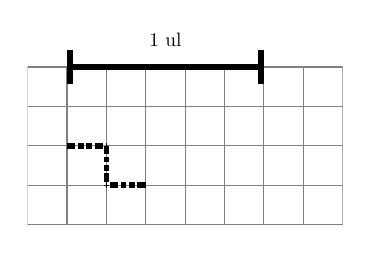
\begin{tikzpicture}[baseline,scale = 0.5]

    \tikzset{
      point/.style={
        thick,
        draw,
        cross out,
        inner sep=0pt,
        minimum width=5pt,
        minimum height=5pt,
      },
    }
    \clip (-1,-0.2) rectangle (7,5);
    	\draw [color={black}] (2.5,4.7) node[anchor = center,scale=0.7, rotate = 0] {1 ul};
	\draw[color ={gray}] (-2,0)--(-2,4);
	\draw[color ={gray}] (-1,0)--(-1,4);
	\draw[color ={gray}] (0,0)--(0,4);
	\draw[color ={gray}] (1,0)--(1,4);
	\draw[color ={gray}] (2,0)--(2,4);
	\draw[color ={gray}] (3,0)--(3,4);
	\draw[color ={gray}] (4,0)--(4,4);
	\draw[color ={gray}] (5,0)--(5,4);
	\draw[color ={gray}] (6,0)--(6,4);
	\draw[color ={gray}] (7,0)--(7,4);
	\draw[color ={gray}] (-2,0)--(7,0);
	\draw[color ={gray}] (-2,1)--(7,1);
	\draw[color ={gray}] (-2,2)--(7,2);
	\draw[color ={gray}] (-2,3)--(7,3);
	\draw[color ={gray}] (-2,4)--(7,4);
	\draw[color ={black},line width = 2,|-|] (0,4)--(5,4);
	\draw[color ={black},line width = 2, densely dash dot dot ] (0,2)--(1,2);
	\draw[color ={black},line width = 2, densely dash dot dot ] (1,2)--(1,1);
	\draw[color ={black},line width = 2, densely dash dot dot ] (2,1)--(1,1);

\end{tikzpicture}
}

\newcommand{\tikzfigXsHR}{
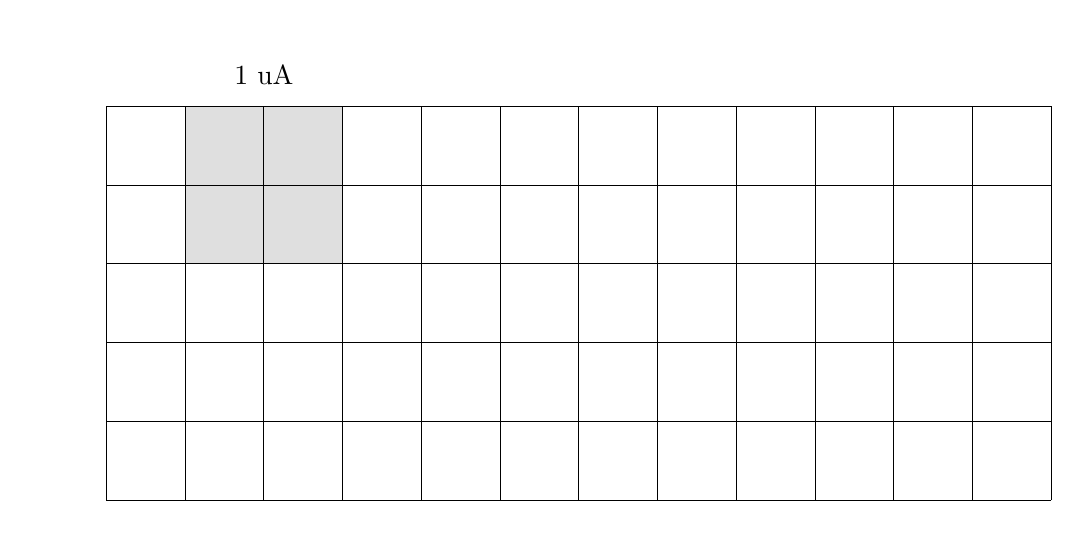
\begin{tikzpicture}[baseline]

    \tikzset{
      point/.style={
        thick,
        draw,
        cross out,
        inner sep=0pt,
        minimum width=5pt,
        minimum height=5pt,
      },
    }
    \clip (-1,-0.1) rectangle (12.1,6);
    	\draw[color={black},preaction={fill,color = {lightgray}, opacity = 0.5}] (1,5)--(3,5)--(3,3)--(1,3)--cycle;
	\draw[color ={black}] (0,0)--(0,5);
	\draw[color ={black}] (1,0)--(1,5);
	\draw[color ={black}] (2,0)--(2,5);
	\draw[color ={black}] (3,0)--(3,5);
	\draw[color ={black}] (4,0)--(4,5);
	\draw[color ={black}] (5,0)--(5,5);
	\draw[color ={black}] (6,0)--(6,5);
	\draw[color ={black}] (7,0)--(7,5);
	\draw[color ={black}] (8,0)--(8,5);
	\draw[color ={black}] (9,0)--(9,5);
	\draw[color ={black}] (10,0)--(10,5);
	\draw[color ={black}] (11,0)--(11,5);
	\draw[color ={black}] (12,0)--(12,5);
	\draw[color ={black}] (0,0)--(12,0);
	\draw[color ={black}] (0,1)--(12,1);
	\draw[color ={black}] (0,2)--(12,2);
	\draw[color ={black}] (0,3)--(12,3);
	\draw[color ={black}] (0,4)--(12,4);
	\draw[color ={black}] (0,5)--(12,5);
	\draw [color={black}] (2,5.4) node[anchor = center,scale=1, rotate = 0] {1 uA};

\end{tikzpicture}
}

\newcommand{\tikzfigSabl}{
\begin{tikzpicture}[baseline,scale = 0.7]

    \tikzset{
      point/.style={
        thick,
        draw,
        cross out,
        inner sep=0pt,
        minimum width=5pt,
        minimum height=5pt,
      },
    }
    \clip (-1,-0.5) rectangle (8.5,2.5);
    	\draw[color={black}] (0,0)--(2.5,0)--(2.5,1)--(0,1)--cycle;
	\draw[color={black}] (3,0)--(7,0)--(7,2)--(3,2)--cycle;
	\draw [color={black}] (7.7,1) node[anchor = center,scale=0.7, rotate = 0] {5 cm};
	\draw [color={black}] (5,-0.3) node[anchor = center,scale=0.7, rotate = 0] {8 cm};
	\draw [color={black}] (1.25,-0.3) node[anchor = center,scale=0.7, rotate = 0] {4 cm};
	\draw [color={black}] (5,1) node[anchor = center,scale=0.7, rotate = 0] {A };
	\draw [color={black}] (1.25,0.5) node[anchor = center,scale=0.7, rotate = 0] {B };

\end{tikzpicture}
}

\newcommand{\tikzfigTIsR}{
\begin{tikzpicture}[baseline]

    \tikzset{
      point/.style={
        thick,
        draw,
        cross out,
        inner sep=0pt,
        minimum width=5pt,
        minimum height=5pt,
      },
    }
    \clip (-0.1,-1.5) rectangle (5.1,1.5);
    	\draw[color ={black},|-|] (0,0)--(5,0);
	\draw[color ={red},<->] (0,0.5)--(5,0.5);
	\draw [color={black}] (2.5,1) node[anchor = center,scale=1, rotate = 0] {?};
	\draw[color ={black},|-|] (0,0)--(2.97,0);
	\draw[color ={blue},<->] (0,-1)--(2.97,-1);
	\draw [color={black}] (1.49,-0.5) node[anchor = center,scale=1, rotate = 0] {3,5};
	\draw[color ={green},<->] (2.97,-1)--(5,-1);
	\draw [color={black}] (3.99,-0.5) node[anchor = center,scale=1, rotate = 0] {2,4};

\end{tikzpicture}
}

\newcommand{\tikzfigGFpM}{
\begin{tikzpicture}[baseline,scale = 0.8]

    \tikzset{
      point/.style={
        thick,
        draw,
        cross out,
        inner sep=0pt,
        minimum width=5pt,
        minimum height=5pt,
      },
    }
    \clip (-2.5,-1) rectangle (3,5);
    	\draw[color={black}] (-2,0)--(2,0)--(0,3.46)--cycle;
	\draw [color={black}] (0,-0.5) node[anchor = center,scale=1, rotate = 0] {5,3 cm};
	\draw [color={red}] (0,0) node[anchor = center,scale=1, rotate = 0] {//};
\draw [color={red}] (1,1.73) node[anchor = center,scale=1, rotate = -60] {//};
\draw [color={red}] (-1,1.73) node[anchor = center,scale=0.5, rotate = -300] {//};


\end{tikzpicture}
}

\newcommand{\tikzfigPROz}{
\begin{tikzpicture}[baseline]

    \tikzset{
      point/.style={
        thick,
        draw,
        cross out,
        inner sep=0pt,
        minimum width=5pt,
        minimum height=5pt,
      },
    }
    \clip (-0.1,-1.5) rectangle (5.1,1.5);
    	\draw[color ={black},|-|] (0,0)--(5,0);
	\draw[color ={green},<->] (0,0.5)--(5,0.5);
	\draw [color={black}] (2.5,1) node[anchor = center,scale=1, rotate = 0] {71};
	\draw[color ={black},|-|] (0,0)--(1.97,0);
	\draw[color ={blue},<->] (0,-1)--(1.97,-1);
	\draw [color={black}] (0.99,-0.5) node[anchor = center,scale=1, rotate = 0] {28};
	\draw[color ={red},<->] (1.97,-1)--(5,-1);
	\draw [color={black}] (3.49,-0.5) node[anchor = center,scale=1, rotate = 0] {?};

\end{tikzpicture}
}

\newcommand{\tikzfigauTD}{
\begin{tikzpicture}[baseline]

    \tikzset{
      point/.style={
        thick,
        draw,
        cross out,
        inner sep=0pt,
        minimum width=5pt,
        minimum height=5pt,
      },
    }
    \clip (-0.1,-1.5) rectangle (5.1,1.5);
    	\draw[color ={black},|-|] (0,0)--(5,0);
	\draw[color ={red},<->] (0,0.5)--(5,0.5);
	\draw [color={black}] (2.5,1) node[anchor = center,scale=1, rotate = 0] {?};
	\draw[color ={black},|-|] (0,0)--(1.8,0);
	\draw[color ={blue},<->] (0,-1)--(1.8,-1);
	\draw [color={black}] (0.9,-0.5) node[anchor = center,scale=1, rotate = 0] {22};
	\draw[color ={green},<->] (1.8,-1)--(5,-1);
	\draw [color={black}] (3.4,-0.5) node[anchor = center,scale=1, rotate = 0] {39};

\end{tikzpicture}
}



\hypersetup{
    pdfauthor={R.Deschamps},
    pdfsubject={},
    pdfkeywords={},
    pdfproducer={LuaLaTeX},
    pdfcreator={Boum Factory}
}
% Activer ou désactiver l'affichage des boîtes
\displayitempointsfalse % Ne pas afficher les boîtes
%\displayitempointstrue % Afficher les boîtes
\newcounter{tourcounter}
\newcommand{\mescartes}[5]{%
    \begin{minipage}{0.237\linewidth}
        \begin{tcolorbox}[
            width=0.85\linewidth, 
            height=4.5cm, 
            colframe=#1, 
            colback=#1!5, 
            colbacktitle=#1!20, 
            title={\textbf{#2}}, 
            sharp corners=all
        ]
            #3
        \end{tcolorbox}
    \end{minipage}
    \hfill
    \begin{minipage}{0.237\linewidth}
        \begin{tcolorbox}[
            width=0.85\linewidth, 
            height=4.5cm, 
            colframe=#1, 
            colback=#1!5, 
            colbacktitle=#1!20, 
            title={\textbf{#4}}, 
            sharp corners=all
        ]
            #5
        \end{tcolorbox}
    \end{minipage}
}
\newcommand{\mesTutocartes}[5]{%
    \begin{minipage}{0.485\linewidth}
        \begin{tcolorbox}[
            width=\linewidth, 
            height=2.5cm, 
            left=0.1pt,
            right=0.1pt,
            colframe=#1, 
            colback=#1!5, 
            colbacktitle=#1!20, 
            title={\color{black}\textbf{#2}}, 
            sharp corners=all
        ]
            #3
        \end{tcolorbox}
    \end{minipage}
    \hfill
    \begin{minipage}{0.485\linewidth}
        \begin{tcolorbox}[
            width=\linewidth, 
            height=2.5cm,  
            left=0.1pt,
            right=0.1pt,
            colframe=#1, 
            colback=#1!5, 
            colbacktitle=#1!20, 
            title={\color{black}\textbf{#4}}, 
            sharp corners=all
        ]
            #5
        \end{tcolorbox}
    \end{minipage}
}
\newcommand{\curseur}[2]{% 1: Couleur, 2: Numéro de l'équipe
    \begin{tikzpicture}[scale=1]
        % Curseur flèche vers la gauche
        \fill[#1] (-2,0) -- (0,1) -- (-0.5,0) -- (0,-1) -- cycle;
        \draw[thick, black] (-2,0) -- (0,1) -- (-0.5,0) -- (0,-1) -- cycle;
        
        % Bulle
        \fill[#1!50] (0.5,0) circle (1);
        \draw[thick, black] (0.5,0) circle (1);
        
        % Queue de la bulle
        \fill[#1!50] (0,0) -- (0.2,-0.2) -- (0.4,0.1) -- cycle;
        %\draw[thick, black] (0,0) -- (0.2,-0.2) -- (0.4,0.1) -- cycle;
        
        % Texte du numéro d'équipe
        \node at (0.5,0) {\textbf{\Huge #2}};
    \end{tikzpicture}
}
\usepackage{tikz}
\usetikzlibrary{shadings,calc} % 'pgfmath' est généralement chargé par défaut
\usepackage{pgfmath}
\tcbuselibrary{skins}

\begin{document}

\setcounter{pagecounter}{0}
\setcounter{ExoMA}{0}
\setcounter{prof}{0}

\def\points{1}
\def\difficulty{1}
\chapitre[
    $\mathbf{6^{\text{ème}}}$% : $\mathbf{6^{\text{ème}}}$,$\mathbf{5^{\text{ème}}}$,$\mathbf{4^{\text{ème}}}$,$\mathbf{3^{\text{ème}}}$,$\mathbf{2^{\text{nde}}}$,$\mathbf{1^{\text{ère}}}$,$\mathbf{T^{\text{Le}}}$,
    ]{
    Liaison CM2-6ème% : ,Equations
    }{
    Collège% : Collège,Lycée
    }{
    %Amadis Jamyn% : Amadis Jamyn,Eugène Belgrand
    }{
    % : ,\tableauPresenteEvalSixieme{}{10},\tableofcontents
    }{
    Activité : % : Exercices
    }
\setrdcrep{seyes, correction=true, correction color=monrose, correction font = \large\bfseries}

\tableofcontents

\newpage

\section{Expression littérale}
\begin{Definition}[Expression littérale]
    Une \voc{expression littérale} est une expression mathématique contenant une ou plusieurs lettres qui désignent des nombres.\\

    Les lettres sont appelées des \voc{variables}.
\end{Definition}
\begin{Exemple}[Expression numérique]
    \begin{multicols}{2}
        \[A=5+7=12\]
        \[B=(-5)\times 7=-35\]
        \[C=\dfrac{5}{2}-\dfrac{2}{3}=\dfrac{5\times 3}{2\times 3}- \dfrac{2\times 2}{3\times 2}=\dfrac{15}{6}-\dfrac{4}{6}=\dfrac{11}{6}\]
        \[D=10^{2}\times 10^{5}=10^{7}\]
    
    
    \columnbreak

        Toutes ces expressions sont composées uniquement de \acc{nombres}, ce sont des \acc{expressions numériques}
    \end{multicols}
\end{Exemple}
\begin{Exemple}[Expression littérale]
    \begin{multicols}{2}
    \begin{enumerate}
        \item La longueur $c$ d’un cercle de rayon $r$ est donnée par : \\
        $c = 2\times {\color{red}\pi} \times \color{blue}r$ 
        où $\color{red}\pi\approx \color{red}3{,}14$…
        \begin{center}
            \figureLongueurCercle
        \end{center}
        Cette formule comporte \acc{une variable}
        \columnbreak

        \item L’aire d’un carré est donné par $\mathbf{\color{blue}c\times c}$
        où $\mathbf{\color{blue}c}$ représente le \acc{côté du carré}.
        \vspace{-0.8cm}\begin{center}
            \figureAireCarre
        \end{center}
    \end{enumerate}
    
    
    \end{multicols}
    \begin{enumerate}[start=3]
        \item Dans l'égalité $6x+6y+7z=21$, il y a \acc{trois variables} : $x ; y \text{ et } z$.\\
    \end{enumerate}
    \solEquation
\end{Exemple}
\newpage
\section{Valeur d’une expression littérale}

\subsection{\'Evaluer une expression littérale}

\begin{Definition}[\'Evaluer une expression littérale]
    \voc{\'Evaluer une expression} littérale signifie \acc{attribuer} une \acc{valeur numérique} à une ou plusieurs \acc{variables}.

    Il s'agit ensuite de \acc{remplacer} ces variables par les valeurs numériques, puis d'\acc{effectuer les calculs} rendus possibles.\\
\end{Definition}

\begin{Methode}
    \begin{minipage}[t]{0.475\textwidth}
        \'Evaluer l'expression suivante pour $x = 5$
        \[A = 2x + t + 3\]

        \textbf{Solution :}\\
        On \acc{remplace} les variables $x$ par $5$ :\\
        \[A = 2\times 5 + t + 3 \quad \text{t n'est pas évaluée}\]
        \[A = 10 + t + 3\]
        \[A = 13 + t\]
    \end{minipage}
    \hfill
    \begin{minipage}[t]{0.475\textwidth}
        Evaluer l'expression suivante pour $x = -1$

        \[B = x + (1 - x) + 3x\]

        \textbf{Solution :}\\
        On \acc{remplace} les variables $x$ par $-1$ :\\
        \[B = -1 + (1 - (-1)) + 3\times ( -1 )\]
        \[B = -1 + (1 + 1) - 3\]
        \[B = -1 + 2 - 3\]
        \[B = -2\]
    \end{minipage}
\end{Methode}

\begin{Remarque}
    \bcattention Penser à rajouter les signes $\times$ lorsqu'on remplace une variable qui est multipliée à un nombre.\\
    \bcattention Les variables ayant des valeurs négatives peuvent être placées \acc{entre parenthèses} pour éviter les erreurs de calcul.
\end{Remarque}

\def\points{8}
\begin{EXO}{\'Evaluer une expression littérale}{C4L13}
    Calculer la valeur des expressions suivantes pour les valeurs données :
    \begin{enumerate}
        \begin{minipage}{0.4\textwidth}\item $A=6\times (x+3)$ lorsque $x=5$
            \vspace{-0.25cm}\begin{crep}
                \[A = 6\times (5+3)\]
                \[A = 6\times 8\]
                \[A = 48\]
            \end{crep}
        \end{minipage}
        \hfill
        \begin{minipage}{0.475\textwidth}\item $B=l\times L$ lorsque $l=3{,}5$ et $L=7$
            \vspace{-0.25cm}\begin{crep}
                \[B = l\times L\]
                \[B = 3{,}5\times 7\]
                \[B = 24{,}5\]
            \end{crep}
        \end{minipage}
        \begin{minipage}{0.4\textwidth}\item $C=5\times(6-x) + 3x -7y$ lorsque $x=2$ et $y=1$
            \vspace{-0.25cm}\begin{crep}
                \[C = 5\times(6-2) + 3\times 2 -7\times 1 \]
                \[C = 5\times(4) + 6 -7 \]
            \end{crep}
        \end{minipage}
        \hfill
        \begin{minipage}{0.475\textwidth}
            \begin{crep}
                \[C = 20 - 1\]
                \[C = 19\]
            \end{crep}
        \end{minipage}
    \end{enumerate}
    
\end{EXO}

\subsection{Nature d'une égalité}
\begin{Definition}
    Une égalité est constituée de deux expressions mathématiques appelées « \voc{membres} » séparées par un signe « = ».
\end{Definition}
\begin{Vocabulaire}[Nature d'une égalité]

    \begin{center}
        \begin{tcbtab}[Une égalité peut être :]{c|c|c|c}
            \voc{Nature de l'égalité}& \acc{Vraie} & \acc{Fausse} & \acc{Parfois vraie, parfois fausse} \\
            \hline
            \acc{Exemple} 1 & $3^2 = (-3)^2$ & $\dfrac{1}{3}=0{,}33$ & $2x=10$ \\
            \acc{Exemple} 2 & $x+x=2x$ & $x^2=-1$ & $3x+1=5x-4$ 
        \end{tcbtab}
    \end{center}
\end{Vocabulaire}
\begin{Exemple}
    \vspace{-0.25cm}\begin{enumerate}
    \item L'égalité $5\times 2=6+4$ est \repsim[3cm]{vraie}, car \repsim[6cm]{$5\times 2=10$ et $6+4=10$}.\\
    \item L'égalité $4\times 6=24+3$ est \repsim[3cm]{fausse}, car \repsim[6cm]{$4\times 6=24$ mais $24+3=27$}.
    \item L'égalité $4x + 6 +2x = 2x\times 3 +2\times 3$ est \repsim[3cm]{vraie} car :
        \begin{crep}
            \begin{minipage}[t]{0.475\textwidth}
                D'une part : \\
                $4x + 6 + 2x = 6x + 6$
            \end{minipage}
            \hfill
            \begin{minipage}[t]{0.475\textwidth}
                D'autre part :\\
                $2x \times 3 + 2 \times 3 = 6x + 6$
            \end{minipage}\\\\
            Les membres de gauche et de droite sont tous les deux égaux à la même \acc{expression littérale} $6x + 6$.\\
            On en déduit que cette égalité est vraie quelle que soit la valeur de $x$.
        \end{crep}
    \end{enumerate}
\end{Exemple}
\def\points{6}
\def\rdifficulty{2}
\begin{EXO}{Déterminer la nature d'une égalité}{C4L14}
    \vspace{-0.25cm}\begin{enumerate}
    $3x+6=2(x+5)$ est \repsim[3cm]{fausse} car :
    \begin{crep}
        \begin{minipage}[t]{0.475\textwidth}
            D'une part : \\
            $2(x + 5) = 2x + 10$
        \end{minipage}
        \hfill
        \begin{minipage}[t]{0.475\textwidth}
            D'autre part :\\
            $3x + 6 \neq 2x + 10$
        \end{minipage}\\\\
        Les deux membres ne sont pas égaux.
    \end{crep}

    \vspace{-0.25cm}$x^{2}=2x$ est \repsim[3cm]{fausse} car :
    \begin{crep}
        Les deux membres ne sont pas égaux pour toutes les valeurs de $x$ : \\
        Si x = 3 par exemple, alors : $x^2 = 3^2 = 9$ mais $2x = 2\times 3 =6$
    \end{crep}
    \end{enumerate}
\end{EXO}
\vspace{-0.25cm}\begin{Remarque}
    Parfois ces égalités, par exemple $3x+5=7$ ou $4x+4=7x+2$, peuvent être égales pour certaines valeurs de $x$, on parle d'équation.
\end{Remarque}

\newpage
\section{Développement}
\subsection{Introduction}
\begin{Activite}[Les bouteilles]
    Un restaurateur a commandé 3 caisses de jus d’orange et 5 caisses de jus de raisin.\\
    Chaque caisse contient 24 bouteilles de jus.\\
    \begin{enumerate}
        \item Répondre à la question suivante de \acc{deux façons différentes} :\\
            \textbf{Combien a-t-il commandé de bouteilles en tout ?}
        \item Que remarque-t-on ?
    \end{enumerate}
    \tcblower
    \begin{enumerate}
        \item \begin{minipage}[t]{0.475\textwidth}
            \acc{Première solution :}
            \begin{crep}
                Le restaurateur a commandé $3\times\blue{24}=72$ bouteilles de jus d'orange.\\
                Il a également commandé $5\times\blue{24}=120$ bouteilles de jus de raisin.\\
                Le nombre total de bouteilles s'écrit :\\
                $3\times \blue{24} + 5 \times \blue{24} = 72 + 120 = 192$ bouteilles.
            \end{crep}
        \end{minipage}
        \hfill
        \begin{minipage}[t]{0.475\textwidth}
            \acc{Seconde solution :}
            \begin{crep}
                Puisque les caisses contiennent le même nombre de bouteilles, il suffit de \acc{multiplier} le nombre de caisses \acc{au total} par le nombre de \acc{bouteilles} par caisse : \\
                $( 3 + 5 ) \times \blue{24} = 8 \times \blue{24} = 192$ bouteilles.
            \end{crep}
        \end{minipage}

        \item On remarque que...\begin{crep}
            L'égalité suivante est vraie : \\
            $( 3 + 5 ) \times \blue{24} = 3\times \blue{24} + 5 \times \blue{24}$
        \end{crep}
    \end{enumerate}
    
\end{Activite}
\subsection{Distributivité}
\begin{Propriete}[Distributivité simple]
    On considère trois expressions ( numériques ou littérales ) a, b et c. \\
    Les égalités suivantes sont \acc{toujours vérifiées} :\\
    \begin{minipage}[t]{0.475\textwidth}
        \begin{center}\Large$\blue{a}(\red{b}+\red{c})=\blue{a}\red{b}+\blue{a}\red{c}$\end{center}
    \end{minipage}
    \hfill
    \begin{minipage}[t]{0.475\textwidth}
        \begin{center}\Large$\blue{a}(\red{b}-\red{c})=\blue{a}\red{b}-\blue{a}\red{c}$\end{center}
    \end{minipage} 
\end{Propriete}

\begin{Exemple}[Calculs astucieux]
    \vspace{-0.35cm}
    \begin{minipage}[t]{0.3\textwidth}\bclampe Pour calculer astucieusement, on peut utiliser la \voc{distributivité}.\end{minipage}
    \hfill
    \begin{minipage}[t]{0.6\textwidth}
    Puisque $101 = 100 + 1$, on peut écrire :
    \[\blue{32} \times 101 = \blue{32} \times (\red{100} + \red{1}) = \blue{32} \times \red{100} + \blue{32} \times \red{1} = 3\,200 + 32 = \color{\currentAccentColor}{3\,232}\]
    \end{minipage}\\

    %\acc{Calculer astucieusement :}\\
    $32\times 99=\tcfillcrep{\blue{32} \times (\red{100} - \red{1}) = \blue{32} \times \red{100} - \blue{32} \times \red{1} = 3\,200 - 32 = 3\,168}$\\
    $13\times 102=\tcfillcrep{\blue{13} \times (\red{100} + \red{2}) = \blue{13} \times \red{100} + \blue{13} \times \red{2} = 1\,300 + 26 = 1\,326}$\\
    $29\times 999=\tcfillcrep{\blue{29} \times (\red{1\,000} - \red{1}) = \blue{29} \times \red{1\,000} - \blue{29} \times \red{1} = 29\,000 - 29 = 28\,971}$
\end{Exemple}
\begin{Definition}[Développer une expression]
    \voc{Développer}, c’est transformer un \acc{produit} en \acc{somme} (ou \acc{différence}).\\
    Dans la pratique, développer c’est lire la formule de distributivité \acc{de la gauche vers la droite}.
\end{Definition}
\begin{Exemple}
    \bclampe Pour \acc{développer} une expression, il suffit de lire la formule de distributivité \acc{de la gauche vers la droite}.\\
    \textbf{L'expression} $A = 4(5+x)$ est un \voc{produit}. \\
    On peut le développer en : 
    $A = \blue{4}(\red{5}+\red{x}) = \blue{4}\times\red{5}+\blue{4}\times\red{x}$
\end{Exemple}

\def\points{4}
\def\rdifficulty{1}
\begin{EXO}{Développer avec la simple distributivité}{C4L21}
    Développe les expressions suivantes :
    \vspace{-0.35cm}\begin{multicols}{2}
        \begin{enumerate}
            \item $A = 5(x-2)$\begin{crep}
            $A = \blue{5}(\red{x}-\red{2}) \\= \blue{5}\times\red{x}-\blue{5}\times\red{2}\\ = 5x - 10$
            \end{crep}
            \item $B = -6(-2x+4)$\begin{crep}
            $B = \blue{-6}(\red{-2x}+\red{4}) \\= \blue{-6}\times\red{(-2x)}+\blue{(-6)}\times\red{4} \\= 12x - 24$
            \end{crep}
        \end{enumerate}
    \end{multicols}
    \begin{multicols}{2}
        \begin{enumerate}[start=3]
            \item $C = -x(2-3x)$\begin{crep}
            $C = \blue{-x}(\red{2}-\red{3x}) \\= \blue{-x}\times\red{2}-\blue{-x}\times\red{(-3x)} \\= -2x - 3x^2$
            \end{crep}
            \item $D = -(5-x)$\begin{crep}
            $D = \blue{-}(\red{5}-\red{x}) \\= \blue{-1}\times\red{5}-\blue{(-1)}\times\red{x} \\= -5 + x$
            \end{crep}
        \end{enumerate}
    \end{multicols}
\end{EXO}

\subsection{Réduire une expression}
\begin{Definition}[Réduire une expression]
    \voc{Réduire} une expression, c’est l’écrire avec le moins de termes ou de facteurs possibles. \\
    Pour cela on \acc{regroupe} les termes de \acc{même nature}. 
\end{Definition}
\begin{Exemple}
    \vspace{-0.25cm}
    \begin{multicols}{2}
        \acc{Réduire} les expressions suivantes :
        \begin{enumerate}
            \item $A = 4x+3x = \repsim[3cm]{7x}$
            \item $B = 2a+4-3a+6-2a+8a-8\\B = \repsim{5}\times a + \repsim{2}$
        \end{enumerate}
    \end{multicols}
    \vspace{-0.25cm}
    \begin{enumerate}[start=3]
        \item $C= x^{2}+8x-7-8x+15-2x^{2}+3x = \repsim[5cm]{-x^2 + 3x + 8}$
    \end{enumerate}
\end{Exemple}
\newpage
\def\points{6}
\def\rdifficulty{2.5}
\begin{EXO}{Développer et réduire des expressions}{C4L22}
    \vspace{-0.25cm}
    \begin{multicols}{2}
        \acc{Développer et réduire} les expressions suivantes :
        \begin{enumerate}
            \item $A=7(x+2)+6(x+3)\\
             A = \repsim[5cm]{7x + 7\times 2 + 6x + 6 \times 3}\\
             A = \repsim[5cm]{13x + 14 + 18}\\
             A = \repsim[3cm]{13x + 32}$

            \columnbreak


            \item $B=-2(-x+3) + 2(x-5)\\
             B = \repsim[5cm]{2x -6 + 2x - 10}\\
             B = \repsim[3cm]{4x-16}$
            \item $C= 7-2(x-2) = \repsim[5cm]{7 - 2x + 4}\\
             C = \repsim[3cm]{-2x + 11}$
        \end{enumerate}
    \end{multicols}
\end{EXO}  

\section{Factorisation}

\begin{Definition}
    \voc{Factoriser}, c’est transformer une \voc{somme} (ou \voc{différence}) en \acc{produit}.\\
    Une expression factorisée est formée de \voc{facteurs}.\\
    Dans la pratique, \acc{factoriser} c’est lire la formule de distributivité \acc{de la droite vers la gauche} : \\
    \begin{minipage}[t]{0.475\textwidth}
        \begin{center}\Large$\blue{a}\red{b}+\blue{a}\red{c}=\blue{a}(\red{b}+\red{c})$\end{center}
    \end{minipage}
    \hfill
    \begin{minipage}[t]{0.475\textwidth}
        \begin{center}\Large$\blue{a}\red{b}-\blue{a}\red{c}=\blue{a}(\red{b}-\red{c})$\end{center}
    \end{minipage} 
\end{Definition}

\begin{Exemple}
    \bclampe \includegraphics[]{images/Factorisation.jpg}
    \acc{Factoriser} les expressions suivantes puis les \voc{simplifier} le plus possible :\\
\end{Exemple}

\begin{EXO}{Factoriser des expressions}{C4L26}
    \begin{multicols}{2}
    \begin{enumerate}
        \item $A=131\times13 + 131\times87\\A=\repsim[5cm]{131 \times (13  + 87)}\\A =\repsim[3cm]{131 \times 100} = \repsim[2.5cm]{13\,100}$
        \item $B=37\times13-37\times3\\B=\repsim[5cm]{37 \times (13  - 3)}\\B =\repsim[3cm]{37 \times 10} = \repsim[2.5cm]{370}$
        \item $C=4x-4\times 5 =\repsim[5cm]{4 \times (x  -5)}$
        \item $D=24-8x =\repsim[5cm]{8 \times (3  - x)}$
        \item $E=7x+42 =\repsim[5cm]{7 \times (x + 6)}$
        \item $F=3x-3 = \repsim[5cm]{3 \times (x  - 1)}$
        \item $G=x^{2}+3x =\repsim[5cm]{x \times (x  + 3 )}$
        \item $H=3x^{2}+6x =\repsim[5cm]{3x \times (x  + 2)}$
    \end{enumerate}
\end{multicols}
\end{EXO}

\newpage
%\vspace{-1.3cm}
\section{Distributivité double}
\begin{Propriete}[Double distributivité]
    Lorsqu'on utilise la distributivité et que les deux facteurs sont des sommes ou des différences de plusieurs termes, il est \acc{utile} de connaître l'égalité suivante : \\
    \[\Large(a+b)(c+d)=ac+ad+bc+bd\]
\end{Propriete}
\begin{Demonstration}
    \begin{crep}
        \begin{minipage}[t]{0.475\textwidth}
            Notons $m = a + b$. \\
            On a alors : $(a +b)(c + d) = m (c + d)$\\
            On applique la \acc{distributivité simple} au membre de droite de l'égalité :\\
            \[\blue{m} (c + d) = \blue{m} \times c + \blue{m} \times d
            = \underbrace{\blue{( a + b )} \times c}_{\text{terme 1}} + \underbrace{\blue{( a + b )} \times d}_{\text{terme 2}}\]\\
            
        \end{minipage}
        \hfill
        \begin{minipage}[t]{0.475\textwidth}
            On développe une nouvelle fois en utilisant la distributivité pour les termes $( a + b ) \times c$ et $( a + b ) \times d$ :\\
            $
                \red{( a + b ) \times c} + \blue{( a + b ) \times d} \\= \red{a \times c + b \times c} + \blue{a \times d + b \times d}
            $\\
            Finalement, on a montré que :\\
            $(a +b)(c + d) = a \times c + b \times c + a \times d + b \times d$
        \end{minipage}
    \end{crep}
\end{Demonstration}
\vspace{-0.4cm}\begin{Remarque}
    \bclampe Comme pour la formule de distributivité simple, il est possible de lire ces formules :
    \begin{itemize}
        \item De la gauche vers la droite pour \acc{développer}.
        \item De la droite vers la gauche pour \acc{factoriser}.
    \end{itemize}
    On a aussi les formules suivantes, qu'il est possible de démontrer en utilisant \acc{les règles des signes}.
    \vspace{-0.65cm}
    \begin{multicols}{2}
        \begin{enumerate}
            \item $(a-b)(c+d)=ac+ad-bc-bd$
            \item $(a-b)(c-d)=ac-ad-bc+bd$
        \end{enumerate}
    \end{multicols}
\end{Remarque}
\def\points{8}
\def\rdifficulty{3}
\vspace{-0.5cm}\begin{EXO}{Utiliser la double distributivité}{C4L24}
    \acc{Développe et réduis} les expressions suivantes :\\
    \vspace{-0.75cm}\begin{multicols}{2}
        \begin{enumerate}
            \item $A = (2x+3)(x+8)\\
            A = \repsim[8cm]{2x\times x + 2x \times 8 + 3 \times x + 3 \times 8}\\
            A = \repsim[8cm]{2x^2 + 19x + 24}$\\
            \item $B = (-3+x)(4-5x)\\
            B = \repsim[8cm]{-3\times 4 + (-3) \times (-5x) + x \times 4 + x \times (-5x)}\\
            B = \repsim[8cm]{-5x^2 + 19x - 12}$
        \end{enumerate}
    \end{multicols}
    \vspace{-0.75cm}\begin{multicols}{2}
        \begin{enumerate}[start=3]
            \item $C = 2(3+x)(3-2x)\\
            C = \repsim[8cm]{(6+2x)(3-2x)}\\
            C = \repsim[8cm]{6\times 3 + 6 \times (-2x) + 2x \times 3 + 2x \times (-2x)}\\
            C = \repsim[8cm]{-4x^2 - 6x + 18}$\\
            \item $D = 2x(1-x)-(x-3)(3x+2)\\
            D = \repsim[8cm]{{\red{2x - 2x^2}} - ( {\blue{3x^2 + 2x - 9x - 6}})}\\
            D = \repsim[8cm]{-2x^2 + 2x - 3x^2 - 2x + 9x + 6}\\
            D = \repsim[8cm]{-5x^2 + 9x + 6}$\\
        \end{enumerate}
    \end{multicols}
\end{EXO}% : \section{Expression littérale}
\begin{Definition}[Expression littérale]
    Une \voc{expression littérale} est une expression mathématique contenant une ou plusieurs lettres qui désignent des nombres.\\

    Les lettres sont appelées des \voc{variables}.
\end{Definition}
\begin{Exemple}[Expression numérique]
    \begin{multicols}{2}
        \[A=5+7=12\]
        \[B=(-5)\times 7=-35\]
        \[C=\dfrac{5}{2}-\dfrac{2}{3}=\dfrac{5\times 3}{2\times 3}- \dfrac{2\times 2}{3\times 2}=\dfrac{15}{6}-\dfrac{4}{6}=\dfrac{11}{6}\]
        \[D=10^{2}\times 10^{5}=10^{7}\]
    
    
    \columnbreak

        Toutes ces expressions sont composées uniquement de \acc{nombres}, ce sont des \acc{expressions numériques}
    \end{multicols}
\end{Exemple}
\begin{Exemple}[Expression littérale]
    \begin{multicols}{2}
    \begin{enumerate}
        \item La longueur $c$ d’un cercle de rayon $r$ est donnée par : \\
        $c = 2\times {\color{red}\pi} \times \color{blue}r$ 
        où $\color{red}\pi\approx \color{red}3{,}14$…
        \begin{center}
            \figureLongueurCercle
        \end{center}
        Cette formule comporte \acc{une variable}
        \columnbreak

        \item L’aire d’un carré est donné par $\mathbf{\color{blue}c\times c}$
        où $\mathbf{\color{blue}c}$ représente le \acc{côté du carré}.
        \vspace{-0.8cm}\begin{center}
            \figureAireCarre
        \end{center}
    \end{enumerate}
    
    
    \end{multicols}
    \begin{enumerate}[start=3]
        \item Dans l'égalité $6x+6y+7z=21$, il y a \acc{trois variables} : $x ; y \text{ et } z$.\\
    \end{enumerate}
    \solEquation
\end{Exemple}
\newpage
\section{Valeur d’une expression littérale}

\subsection{\'Evaluer une expression littérale}

\begin{Definition}[\'Evaluer une expression littérale]
    \voc{\'Evaluer une expression} littérale signifie \acc{attribuer} une \acc{valeur numérique} à une ou plusieurs \acc{variables}.

    Il s'agit ensuite de \acc{remplacer} ces variables par les valeurs numériques, puis d'\acc{effectuer les calculs} rendus possibles.\\
\end{Definition}

\begin{Methode}
    \begin{minipage}[t]{0.475\textwidth}
        \'Evaluer l'expression suivante pour $x = 5$
        \[A = 2x + t + 3\]

        \textbf{Solution :}\\
        On \acc{remplace} les variables $x$ par $5$ :\\
        \[A = 2\times 5 + t + 3 \quad \text{t n'est pas évaluée}\]
        \[A = 10 + t + 3\]
        \[A = 13 + t\]
    \end{minipage}
    \hfill
    \begin{minipage}[t]{0.475\textwidth}
        Evaluer l'expression suivante pour $x = -1$

        \[B = x + (1 - x) + 3x\]

        \textbf{Solution :}\\
        On \acc{remplace} les variables $x$ par $-1$ :\\
        \[B = -1 + (1 - (-1)) + 3\times ( -1 )\]
        \[B = -1 + (1 + 1) - 3\]
        \[B = -1 + 2 - 3\]
        \[B = -2\]
    \end{minipage}
\end{Methode}

\begin{Remarque}
    \bcattention Penser à rajouter les signes $\times$ lorsqu'on remplace une variable qui est multipliée à un nombre.\\
    \bcattention Les variables ayant des valeurs négatives peuvent être placées \acc{entre parenthèses} pour éviter les erreurs de calcul.
\end{Remarque}

\def\points{8}
\begin{EXO}{\'Evaluer une expression littérale}{C4L13}
    Calculer la valeur des expressions suivantes pour les valeurs données :
    \begin{enumerate}
        \begin{minipage}{0.4\textwidth}\item $A=6\times (x+3)$ lorsque $x=5$
            \vspace{-0.25cm}\begin{crep}
                \[A = 6\times (5+3)\]
                \[A = 6\times 8\]
                \[A = 48\]
            \end{crep}
        \end{minipage}
        \hfill
        \begin{minipage}{0.475\textwidth}\item $B=l\times L$ lorsque $l=3{,}5$ et $L=7$
            \vspace{-0.25cm}\begin{crep}
                \[B = l\times L\]
                \[B = 3{,}5\times 7\]
                \[B = 24{,}5\]
            \end{crep}
        \end{minipage}
        \begin{minipage}{0.4\textwidth}\item $C=5\times(6-x) + 3x -7y$ lorsque $x=2$ et $y=1$
            \vspace{-0.25cm}\begin{crep}
                \[C = 5\times(6-2) + 3\times 2 -7\times 1 \]
                \[C = 5\times(4) + 6 -7 \]
            \end{crep}
        \end{minipage}
        \hfill
        \begin{minipage}{0.475\textwidth}
            \begin{crep}
                \[C = 20 - 1\]
                \[C = 19\]
            \end{crep}
        \end{minipage}
    \end{enumerate}
    
\end{EXO}

\subsection{Nature d'une égalité}
\begin{Definition}
    Une égalité est constituée de deux expressions mathématiques appelées « \voc{membres} » séparées par un signe « = ».
\end{Definition}
\begin{Vocabulaire}[Nature d'une égalité]

    \begin{center}
        \begin{tcbtab}[Une égalité peut être :]{c|c|c|c}
            \voc{Nature de l'égalité}& \acc{Vraie} & \acc{Fausse} & \acc{Parfois vraie, parfois fausse} \\
            \hline
            \acc{Exemple} 1 & $3^2 = (-3)^2$ & $\dfrac{1}{3}=0{,}33$ & $2x=10$ \\
            \acc{Exemple} 2 & $x+x=2x$ & $x^2=-1$ & $3x+1=5x-4$ 
        \end{tcbtab}
    \end{center}
\end{Vocabulaire}
\begin{Exemple}
    \vspace{-0.25cm}\begin{enumerate}
    \item L'égalité $5\times 2=6+4$ est \repsim[3cm]{vraie}, car \repsim[6cm]{$5\times 2=10$ et $6+4=10$}.\\
    \item L'égalité $4\times 6=24+3$ est \repsim[3cm]{fausse}, car \repsim[6cm]{$4\times 6=24$ mais $24+3=27$}.
    \item L'égalité $4x + 6 +2x = 2x\times 3 +2\times 3$ est \repsim[3cm]{vraie} car :
        \begin{crep}
            \begin{minipage}[t]{0.475\textwidth}
                D'une part : \\
                $4x + 6 + 2x = 6x + 6$
            \end{minipage}
            \hfill
            \begin{minipage}[t]{0.475\textwidth}
                D'autre part :\\
                $2x \times 3 + 2 \times 3 = 6x + 6$
            \end{minipage}\\\\
            Les membres de gauche et de droite sont tous les deux égaux à la même \acc{expression littérale} $6x + 6$.\\
            On en déduit que cette égalité est vraie quelle que soit la valeur de $x$.
        \end{crep}
    \end{enumerate}
\end{Exemple}
\def\points{6}
\def\rdifficulty{2}
\begin{EXO}{Déterminer la nature d'une égalité}{C4L14}
    \vspace{-0.25cm}\begin{enumerate}
    $3x+6=2(x+5)$ est \repsim[3cm]{fausse} car :
    \begin{crep}
        \begin{minipage}[t]{0.475\textwidth}
            D'une part : \\
            $2(x + 5) = 2x + 10$
        \end{minipage}
        \hfill
        \begin{minipage}[t]{0.475\textwidth}
            D'autre part :\\
            $3x + 6 \neq 2x + 10$
        \end{minipage}\\\\
        Les deux membres ne sont pas égaux.
    \end{crep}

    \vspace{-0.25cm}$x^{2}=2x$ est \repsim[3cm]{fausse} car :
    \begin{crep}
        Les deux membres ne sont pas égaux pour toutes les valeurs de $x$ : \\
        Si x = 3 par exemple, alors : $x^2 = 3^2 = 9$ mais $2x = 2\times 3 =6$
    \end{crep}
    \end{enumerate}
\end{EXO}
\vspace{-0.25cm}\begin{Remarque}
    Parfois ces égalités, par exemple $3x+5=7$ ou $4x+4=7x+2$, peuvent être égales pour certaines valeurs de $x$, on parle d'équation.
\end{Remarque}

\newpage
\section{Développement}
\subsection{Introduction}
\begin{Activite}[Les bouteilles]
    Un restaurateur a commandé 3 caisses de jus d’orange et 5 caisses de jus de raisin.\\
    Chaque caisse contient 24 bouteilles de jus.\\
    \begin{enumerate}
        \item Répondre à la question suivante de \acc{deux façons différentes} :\\
            \textbf{Combien a-t-il commandé de bouteilles en tout ?}
        \item Que remarque-t-on ?
    \end{enumerate}
    \tcblower
    \begin{enumerate}
        \item \begin{minipage}[t]{0.475\textwidth}
            \acc{Première solution :}
            \begin{crep}
                Le restaurateur a commandé $3\times\blue{24}=72$ bouteilles de jus d'orange.\\
                Il a également commandé $5\times\blue{24}=120$ bouteilles de jus de raisin.\\
                Le nombre total de bouteilles s'écrit :\\
                $3\times \blue{24} + 5 \times \blue{24} = 72 + 120 = 192$ bouteilles.
            \end{crep}
        \end{minipage}
        \hfill
        \begin{minipage}[t]{0.475\textwidth}
            \acc{Seconde solution :}
            \begin{crep}
                Puisque les caisses contiennent le même nombre de bouteilles, il suffit de \acc{multiplier} le nombre de caisses \acc{au total} par le nombre de \acc{bouteilles} par caisse : \\
                $( 3 + 5 ) \times \blue{24} = 8 \times \blue{24} = 192$ bouteilles.
            \end{crep}
        \end{minipage}

        \item On remarque que...\begin{crep}
            L'égalité suivante est vraie : \\
            $( 3 + 5 ) \times \blue{24} = 3\times \blue{24} + 5 \times \blue{24}$
        \end{crep}
    \end{enumerate}
    
\end{Activite}
\subsection{Distributivité}
\begin{Propriete}[Distributivité simple]
    On considère trois expressions ( numériques ou littérales ) a, b et c. \\
    Les égalités suivantes sont \acc{toujours vérifiées} :\\
    \begin{minipage}[t]{0.475\textwidth}
        \begin{center}\Large$\blue{a}(\red{b}+\red{c})=\blue{a}\red{b}+\blue{a}\red{c}$\end{center}
    \end{minipage}
    \hfill
    \begin{minipage}[t]{0.475\textwidth}
        \begin{center}\Large$\blue{a}(\red{b}-\red{c})=\blue{a}\red{b}-\blue{a}\red{c}$\end{center}
    \end{minipage} 
\end{Propriete}

\begin{Exemple}[Calculs astucieux]
    \vspace{-0.35cm}
    \begin{minipage}[t]{0.3\textwidth}\bclampe Pour calculer astucieusement, on peut utiliser la \voc{distributivité}.\end{minipage}
    \hfill
    \begin{minipage}[t]{0.6\textwidth}
    Puisque $101 = 100 + 1$, on peut écrire :
    \[\blue{32} \times 101 = \blue{32} \times (\red{100} + \red{1}) = \blue{32} \times \red{100} + \blue{32} \times \red{1} = 3\,200 + 32 = \color{\currentAccentColor}{3\,232}\]
    \end{minipage}\\

    %\acc{Calculer astucieusement :}\\
    $32\times 99=\tcfillcrep{\blue{32} \times (\red{100} - \red{1}) = \blue{32} \times \red{100} - \blue{32} \times \red{1} = 3\,200 - 32 = 3\,168}$\\
    $13\times 102=\tcfillcrep{\blue{13} \times (\red{100} + \red{2}) = \blue{13} \times \red{100} + \blue{13} \times \red{2} = 1\,300 + 26 = 1\,326}$\\
    $29\times 999=\tcfillcrep{\blue{29} \times (\red{1\,000} - \red{1}) = \blue{29} \times \red{1\,000} - \blue{29} \times \red{1} = 29\,000 - 29 = 28\,971}$
\end{Exemple}
\begin{Definition}[Développer une expression]
    \voc{Développer}, c’est transformer un \acc{produit} en \acc{somme} (ou \acc{différence}).\\
    Dans la pratique, développer c’est lire la formule de distributivité \acc{de la gauche vers la droite}.
\end{Definition}
\begin{Exemple}
    \bclampe Pour \acc{développer} une expression, il suffit de lire la formule de distributivité \acc{de la gauche vers la droite}.\\
    \textbf{L'expression} $A = 4(5+x)$ est un \voc{produit}. \\
    On peut le développer en : 
    $A = \blue{4}(\red{5}+\red{x}) = \blue{4}\times\red{5}+\blue{4}\times\red{x}$
\end{Exemple}

\def\points{4}
\def\rdifficulty{1}
\begin{EXO}{Développer avec la simple distributivité}{C4L21}
    Développe les expressions suivantes :
    \vspace{-0.35cm}\begin{multicols}{2}
        \begin{enumerate}
            \item $A = 5(x-2)$\begin{crep}
            $A = \blue{5}(\red{x}-\red{2}) \\= \blue{5}\times\red{x}-\blue{5}\times\red{2}\\ = 5x - 10$
            \end{crep}
            \item $B = -6(-2x+4)$\begin{crep}
            $B = \blue{-6}(\red{-2x}+\red{4}) \\= \blue{-6}\times\red{(-2x)}+\blue{(-6)}\times\red{4} \\= 12x - 24$
            \end{crep}
        \end{enumerate}
    \end{multicols}
    \begin{multicols}{2}
        \begin{enumerate}[start=3]
            \item $C = -x(2-3x)$\begin{crep}
            $C = \blue{-x}(\red{2}-\red{3x}) \\= \blue{-x}\times\red{2}-\blue{-x}\times\red{(-3x)} \\= -2x - 3x^2$
            \end{crep}
            \item $D = -(5-x)$\begin{crep}
            $D = \blue{-}(\red{5}-\red{x}) \\= \blue{-1}\times\red{5}-\blue{(-1)}\times\red{x} \\= -5 + x$
            \end{crep}
        \end{enumerate}
    \end{multicols}
\end{EXO}

\subsection{Réduire une expression}
\begin{Definition}[Réduire une expression]
    \voc{Réduire} une expression, c’est l’écrire avec le moins de termes ou de facteurs possibles. \\
    Pour cela on \acc{regroupe} les termes de \acc{même nature}. 
\end{Definition}
\begin{Exemple}
    \vspace{-0.25cm}
    \begin{multicols}{2}
        \acc{Réduire} les expressions suivantes :
        \begin{enumerate}
            \item $A = 4x+3x = \repsim[3cm]{7x}$
            \item $B = 2a+4-3a+6-2a+8a-8\\B = \repsim{5}\times a + \repsim{2}$
        \end{enumerate}
    \end{multicols}
    \vspace{-0.25cm}
    \begin{enumerate}[start=3]
        \item $C= x^{2}+8x-7-8x+15-2x^{2}+3x = \repsim[5cm]{-x^2 + 3x + 8}$
    \end{enumerate}
\end{Exemple}
\newpage
\def\points{6}
\def\rdifficulty{2.5}
\begin{EXO}{Développer et réduire des expressions}{C4L22}
    \vspace{-0.25cm}
    \begin{multicols}{2}
        \acc{Développer et réduire} les expressions suivantes :
        \begin{enumerate}
            \item $A=7(x+2)+6(x+3)\\
             A = \repsim[5cm]{7x + 7\times 2 + 6x + 6 \times 3}\\
             A = \repsim[5cm]{13x + 14 + 18}\\
             A = \repsim[3cm]{13x + 32}$

            \columnbreak


            \item $B=-2(-x+3) + 2(x-5)\\
             B = \repsim[5cm]{2x -6 + 2x - 10}\\
             B = \repsim[3cm]{4x-16}$
            \item $C= 7-2(x-2) = \repsim[5cm]{7 - 2x + 4}\\
             C = \repsim[3cm]{-2x + 11}$
        \end{enumerate}
    \end{multicols}
\end{EXO}  

\section{Factorisation}

\begin{Definition}
    \voc{Factoriser}, c’est transformer une \voc{somme} (ou \voc{différence}) en \acc{produit}.\\
    Une expression factorisée est formée de \voc{facteurs}.\\
    Dans la pratique, \acc{factoriser} c’est lire la formule de distributivité \acc{de la droite vers la gauche} : \\
    \begin{minipage}[t]{0.475\textwidth}
        \begin{center}\Large$\blue{a}\red{b}+\blue{a}\red{c}=\blue{a}(\red{b}+\red{c})$\end{center}
    \end{minipage}
    \hfill
    \begin{minipage}[t]{0.475\textwidth}
        \begin{center}\Large$\blue{a}\red{b}-\blue{a}\red{c}=\blue{a}(\red{b}-\red{c})$\end{center}
    \end{minipage} 
\end{Definition}

\begin{Exemple}
    \bclampe \includegraphics[]{images/Factorisation.jpg}
    \acc{Factoriser} les expressions suivantes puis les \voc{simplifier} le plus possible :\\
\end{Exemple}

\begin{EXO}{Factoriser des expressions}{C4L26}
    \begin{multicols}{2}
    \begin{enumerate}
        \item $A=131\times13 + 131\times87\\A=\repsim[5cm]{131 \times (13  + 87)}\\A =\repsim[3cm]{131 \times 100} = \repsim[2.5cm]{13\,100}$
        \item $B=37\times13-37\times3\\B=\repsim[5cm]{37 \times (13  - 3)}\\B =\repsim[3cm]{37 \times 10} = \repsim[2.5cm]{370}$
        \item $C=4x-4\times 5 =\repsim[5cm]{4 \times (x  -5)}$
        \item $D=24-8x =\repsim[5cm]{8 \times (3  - x)}$
        \item $E=7x+42 =\repsim[5cm]{7 \times (x + 6)}$
        \item $F=3x-3 = \repsim[5cm]{3 \times (x  - 1)}$
        \item $G=x^{2}+3x =\repsim[5cm]{x \times (x  + 3 )}$
        \item $H=3x^{2}+6x =\repsim[5cm]{3x \times (x  + 2)}$
    \end{enumerate}
\end{multicols}
\end{EXO}

\newpage
%\vspace{-1.3cm}
\section{Distributivité double}
\begin{Propriete}[Double distributivité]
    Lorsqu'on utilise la distributivité et que les deux facteurs sont des sommes ou des différences de plusieurs termes, il est \acc{utile} de connaître l'égalité suivante : \\
    \[\Large(a+b)(c+d)=ac+ad+bc+bd\]
\end{Propriete}
\begin{Demonstration}
    \begin{crep}
        \begin{minipage}[t]{0.475\textwidth}
            Notons $m = a + b$. \\
            On a alors : $(a +b)(c + d) = m (c + d)$\\
            On applique la \acc{distributivité simple} au membre de droite de l'égalité :\\
            \[\blue{m} (c + d) = \blue{m} \times c + \blue{m} \times d
            = \underbrace{\blue{( a + b )} \times c}_{\text{terme 1}} + \underbrace{\blue{( a + b )} \times d}_{\text{terme 2}}\]\\
            
        \end{minipage}
        \hfill
        \begin{minipage}[t]{0.475\textwidth}
            On développe une nouvelle fois en utilisant la distributivité pour les termes $( a + b ) \times c$ et $( a + b ) \times d$ :\\
            $
                \red{( a + b ) \times c} + \blue{( a + b ) \times d} \\= \red{a \times c + b \times c} + \blue{a \times d + b \times d}
            $\\
            Finalement, on a montré que :\\
            $(a +b)(c + d) = a \times c + b \times c + a \times d + b \times d$
        \end{minipage}
    \end{crep}
\end{Demonstration}
\vspace{-0.4cm}\begin{Remarque}
    \bclampe Comme pour la formule de distributivité simple, il est possible de lire ces formules :
    \begin{itemize}
        \item De la gauche vers la droite pour \acc{développer}.
        \item De la droite vers la gauche pour \acc{factoriser}.
    \end{itemize}
    On a aussi les formules suivantes, qu'il est possible de démontrer en utilisant \acc{les règles des signes}.
    \vspace{-0.65cm}
    \begin{multicols}{2}
        \begin{enumerate}
            \item $(a-b)(c+d)=ac+ad-bc-bd$
            \item $(a-b)(c-d)=ac-ad-bc+bd$
        \end{enumerate}
    \end{multicols}
\end{Remarque}
\def\points{8}
\def\rdifficulty{3}
\vspace{-0.5cm}\begin{EXO}{Utiliser la double distributivité}{C4L24}
    \acc{Développe et réduis} les expressions suivantes :\\
    \vspace{-0.75cm}\begin{multicols}{2}
        \begin{enumerate}
            \item $A = (2x+3)(x+8)\\
            A = \repsim[8cm]{2x\times x + 2x \times 8 + 3 \times x + 3 \times 8}\\
            A = \repsim[8cm]{2x^2 + 19x + 24}$\\
            \item $B = (-3+x)(4-5x)\\
            B = \repsim[8cm]{-3\times 4 + (-3) \times (-5x) + x \times 4 + x \times (-5x)}\\
            B = \repsim[8cm]{-5x^2 + 19x - 12}$
        \end{enumerate}
    \end{multicols}
    \vspace{-0.75cm}\begin{multicols}{2}
        \begin{enumerate}[start=3]
            \item $C = 2(3+x)(3-2x)\\
            C = \repsim[8cm]{(6+2x)(3-2x)}\\
            C = \repsim[8cm]{6\times 3 + 6 \times (-2x) + 2x \times 3 + 2x \times (-2x)}\\
            C = \repsim[8cm]{-4x^2 - 6x + 18}$\\
            \item $D = 2x(1-x)-(x-3)(3x+2)\\
            D = \repsim[8cm]{{\red{2x - 2x^2}} - ( {\blue{3x^2 + 2x - 9x - 6}})}\\
            D = \repsim[8cm]{-2x^2 + 2x - 3x^2 - 2x + 9x + 6}\\
            D = \repsim[8cm]{-5x^2 + 9x + 6}$\\
        \end{enumerate}
    \end{multicols}
\end{EXO},



\end{document}